
Os resultados apresentados posteriormente foram gerados usando a base de dados KITTI \cite{Geiger}.
No primeiro teste, mostrado na Figura \ref{fig:imgpapercerta}, o algoritmo busca um objeto 
de interesse numa sequência de
9 imagens, tendo o objeto um deslocamento aproximadamente perpendicular em relação ao observador.
\begin{figure}[!hbt]
\centering
  \subfloat[]{\label{fig:imgpapercertaa} \includegraphics[width=.48\columnwidth]{images/images/0000000000.png}}
  \subfloat[]{\label{fig:imgpapercertab} \includegraphics[width=.48\columnwidth]{images/images/img_paper_certa.eps}}
  \caption{A imagem (a) representa o objeto na sua posição inicial 
   e a imagem (b) mostra o veículo na posição final.}
  \label{fig:imgpapercerta}
\end{figure}

O vetor em azul ilustra o resultando da busca, saindo do ponto inicial até o final. 
Nota-se, também, que existe uma curvatura na foto devido à câmera e, por consequência,
um impacto no resultado. Deste modo, é possível verificar a sensibilidade do algoritmo 
por menor que seja a variação da área do $ROI$, como mostrado na Figura \ref{fig:res_graph1}.

\begin{figure}[!hbt]
\centering
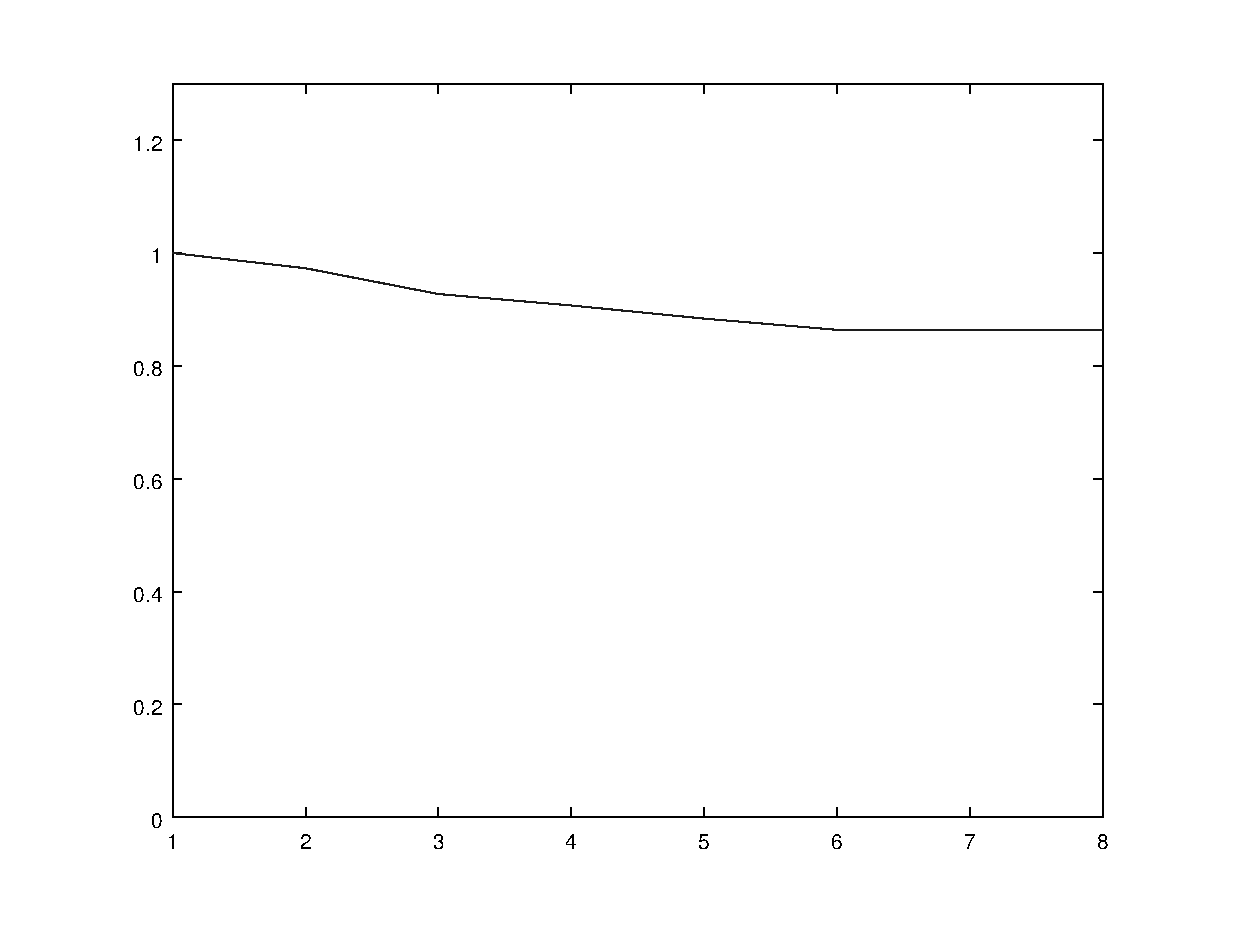
\includegraphics[width=0.8\columnwidth]{images/graph1.eps}
\caption{Fator de aproximação para cada imagem no teste 1.}
\label{fig:res_graph1}
\end{figure}

Na Figura \ref{fig:res_graph1v} observa-se a velocidade com que o fator de aproximação se modifica e, ainda,
é possível constatar a pequena variação no fator de aproximação, se comparado
com o valor de referência 1. A média do fator de aproximação(velocidade) é de $-0.017020$, implicando
em uma aproximação de $1.7\%$ de $d_0$ em cada um das nove imagens.

\begin{figure}[!hbt]
\centering
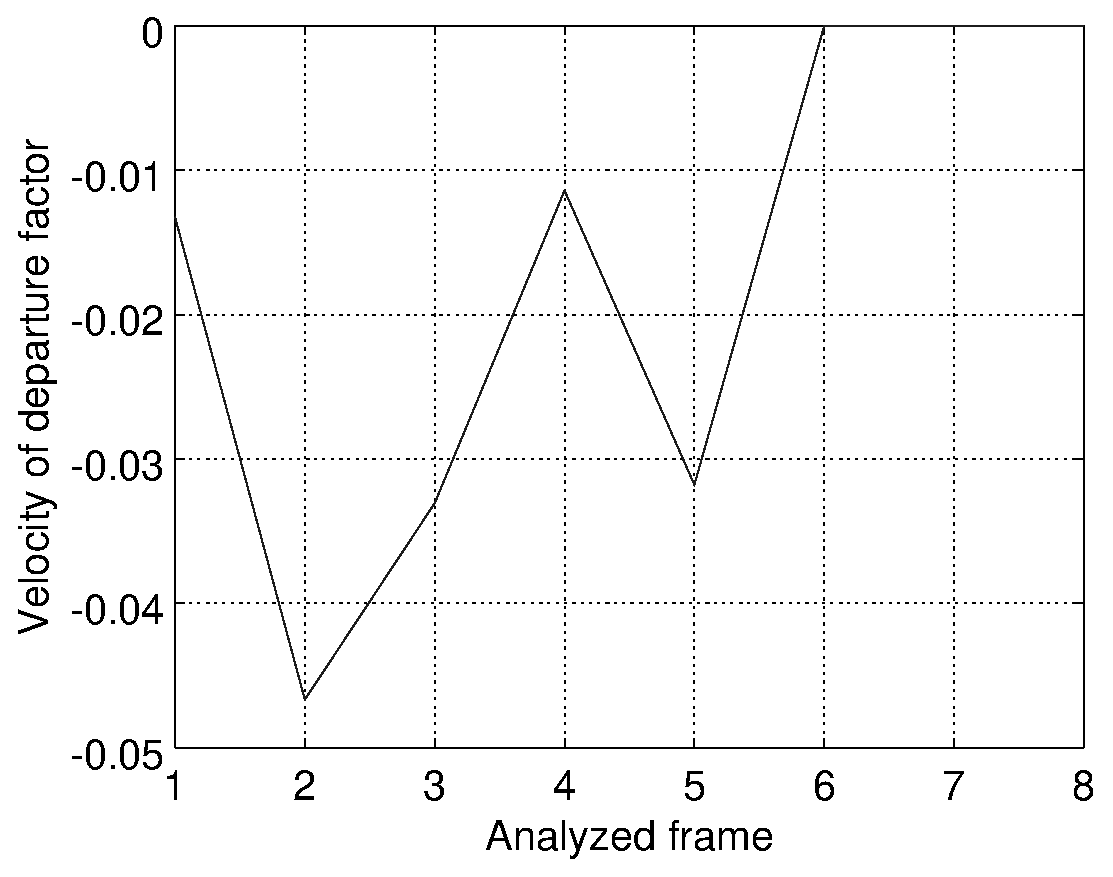
\includegraphics[width=0.8\columnwidth]{images/graph1v.eps}
\caption{Velocity of departure factor for each frame in the test 1.}
\label{fig:res_graph1v}
\end{figure}
